\documentclass[12pt,a4paper,pdftex]{article}

% Sprache
\usepackage[ngerman]{babel}

\usepackage[utf8]{inputenc}

\usepackage{graphicx}

% Page layout
\usepackage{geometry}
\geometry{a4paper,lmargin={2.5cm}, rmargin={2.5cm}, tmargin={2cm}, bmargin={2.5cm}}

% Figure and Caption layout
\usepackage[bf]{caption}
\usepackage{subcaption}
\usepackage{wrapfig}

% Befehle zur Textauszeichnung (hervorheben, unterstreichen ect.)
\usepackage{color,soul}

% Zitier-Style für Bücher und URL
\usepackage[round, authoryear]{natbib}
\usepackage[breaklinks=true,bookmarks=true,bookmarksopen=true,colorlinks=true,citecolor=gray,linkcolor=black,urlcolor=gray,pdfpagemode=UseNone,pdfstartview=FitH]{hyperref}


\usepackage{float}
\usepackage{gensymb}
\usepackage{siunitx}
\usepackage{tabularx}
\usepackage{amsmath}

% for commenting a whole section
\usepackage{verbatim}

\usepackage{pgfgantt}
\usepackage{afterpage}

% Index
\usepackage{imakeidx}
\makeindex[intoc, columnseprule]
\newcommand{\indextitle}{\section{Index}}

% Bilder importieren
\usepackage{epstopdf}
\epstopdfDeclareGraphicsRule{.pdf}{png}{.png}{convert #1 \OutputFile}
\DeclareGraphicsExtensions{.png,.pdf}

% Bildernummerierung fuer jedes kapitel
\usepackage{chngcntr}
\counterwithin{figure}{section}

% ich hab keine ahnung was die tun und wir brauchen sie auch nicht
%\newcommand{\command}[1]{\texttt{#1}}
%\newcommand{\fileextension}[1]{\texttt{#1}}

% plus minus zeichen
\newcommand{\rpm}{\raisebox{.2ex}{$\scriptstyle\pm$} }

% kapitel title auf deutsch
\renewcommand{\bibsection}{\section{Literaturverzeichnis}}



%%%%%%%%%%%%%%%%%%%%%%%%%%%%%%%%%%%%%%%%%%%%%%%%%%%%%%%%%%%%%

\begin{document}
\setlength{\parindent}{0pt}

%%%%%%%%%%%%%%%%%%%%%%%%%%%%%%%%%%%%%%%%%%%%%%%%%%%%%%%%%%%%%
% Titelseite

\begin{titlepage}
 \begin{center}
        \vspace*{1cm}
        \LARGE
        \textbf{Kurzes Lehrbuch der Neuroanatomie des Säugers}
        \vspace{2cm}
        
        \Large
        Praktikumsprotokoll des Mastermoduls Neuroanatomie
        \vspace{4cm}
        
        \large
        vorgelegt von \\ Jacqueline Göbl, Julia Grüb, Marta Provenzano und Laura Seidler % Author name
        \vfill
        \large     
        T\"ubingen, \today
    \end{center}
    \newpage
        \thispagestyle{empty}
        \mbox{}
        \newpage
\end{titlepage}


\thispagestyle{empty}
\mbox{}
%%%%%%%%%%%%%%%%%%%%%%%%%%%%%%%%%%%%%%%%%%%%%%%%%%%%%%%%%%%%%% Inhaltsverzeichnis und Abbildungsverzeichnis

\tableofcontents
\newpage
\listoffigures

%%%%%%%%%%%%%%%%%%%%%%%%%%%%%%%%%%%%%%%%%%%%%%%%%%%%%%%%%%%%%
% Textbeginn

\newpage
\section{Einleitung}
\begin{itemize}
    \item Kurze Geschichte der Anatomie
    \item The thalamus is an egg-shaped cluster of nuclei in the
center of the brain that acts as a center of communica-
tion between many subcortical brain centers and the
neocortex. The locations of nuclei within the thalamus
correspond roughly with the hemispheric locations of
the regions of the cerebral cortex with which they com-
municate \cite[Kap.~22]{kandel2013principles} p.494
\end{itemize}
\newpage
\section{Material und Methoden}

Computerprogramm am Aufnahmecomputer der Bilder:
Axio Vision (AxioVs40 4.8.2.0, Copyright 2006-2010, Carl zeiss MicroImaging GmBH)



\begin{itemize}
    \item Schafhirn - die Präperationsanleitungen hat auch Jacqui
    \item Perfusion der Ratte - hat auch Jacqui
    \item Färbungen (Nissl, Faser, Immunohistochemie)
    \item Auswertung am Mikroskop - Jacqui hat die genauen Angaben des Programms welches wir für die Mikroskopaufnahmen benutzt wurde
\end{itemize}

\newpage
\section{Allgemeine Übersicht}
\subsection{Äußere Morphologie und Hirnteile}

\begin{itemize}
    \item Lage
    \item charakteristische Form
    \item Bezug zum Ventrikelsystem
    \item Differenzierung zwischen Kerngebieten und cortikalen Strukturen
    \item Charakterisierung der Großhirnrinde (Cortex) - Neocortex, Allocortex, Areale, Schichtung, typische Verbindungsmuster
\end{itemize}
\subsection{Spezifische Lage der Hirnnervenkerne im Hirnstamm}
\begin{itemize}
    \item relative Lage in Bezug zu sensorischen und motorischen Funktionen; Bezug zur dorsoventralen Organisation des Rückenmarks  
    (motorische Kerne liegen systematisch  wo anders als somatosensorische Kerne ---wegen der Auflösung der dorsoventralen Struktur zu einer medialen lateralen Struktur) 
    \item sensorisch: N.trigeminus, N.cochlearis, N.vestibularis, NTS
    \item motorisch: Mo5, Mo7, N. ocolomotorius
\end{itemize}

% Allgemeine sensorische Bahnen
\newpage
\section{Allgemeine sensorische Bahnen}
Dieses Kapitel behandelt die allgemeine Sensorik \index{Sensorik !allgemein} die im Gegensatz zu speziellen Sensorik (Kapitel~ \ref{sec:spezsens}) steht. In der allgemeine Sensorik sind die Sinne zusammen gefasst welche über den ganzen Körper verteilt sind, dazu gehören unter anderem die Somatosensorik \index{Sensorik !Somato-} die Propriozeption \index{Propriozeption} und die Viszerosensorik \index{Sensorik !Viszero-}\cite[Kap. 22]{kandel2013principles}. Die spezielle Sensorik \index{Sensorik !speziell} fasst die Sinne zusammen welche auf Grund der Cephalisation bei Säugern nach vorne in den Kopf verlagert sind.
\\
Die Somatosensorik zeichnet sich durch die Repräsentation der direkten äußeren Welt und der inneren Welt aus. Bei der Repräsentation der Außenwelt unterscheidet man bei Säugetieren zwischen zwei Rezeptorsystemen. Zum einen die haarlose Haut in den Handinnenflächen, an der Fußunterseite und an den Lippen und der Nase, zum anderen die behaarte Haut mit hoch spezialisierten Tastsinneszellen innerviert durch die Bewegungen des Follikels auf den Blutsinus \index{Blutsinus} der Vibrissen.  \index{Sinushaar} \cite{paxinos2014rat}
Die Propriozeption codiert die Informationen der relative Position unserer Extremitäten und anderer Körperteile im Raum und bildet in den Vorderextremitäten die Grundlage für abstrakte Wahrnehmung von Objektgrößen und Gewicht. Ein weiteren Bereich in der Somatosensorik bildet der Sinn welcher Schmerzen und Temperatur verarbeitet. \cite{paxinos2014rat}
Im Weiteren wird am Beispiel der Ratte näher auf die unterschiedlichen Systeme eingegangen und wodurch diese sich genau unterscheiden. 

%%%%% comment
\begin{comment}
\begin{itemize}
    \item kurze einführung was Somatosensorik ist und welche Typen unterscheiden werden
    \item kurze reichweite
    \item innere und äußere welt
    \item glabrous skin nur an Hand und Fußinnenflächen und Lippen und Nase \cite{paxinos2014rat} p.675
    \item behaarte Haut \\ However, in rats the most highly
    specialized touch receptors are those that innervate the
    elaborate follicles of the large whiskers on the face (a.k.a.the mystacial vibrissae or sinus hairs) \cite{paxinos2014rat}
    \item Proprioception \\ The study of somatic
    sensation includes both cutaneous mechanisms, and
    another less obvious sense that informs us about where
    our limbs are in space relative to the environment and
    the other parts of our body (proprioception). Proprio-
    ception in the forelimb also forms the basis for abstrac-
    tions such as object size and weight. \cite{paxinos2014rat}
    \item schmerz und temperatur sinn
\end{itemize}
\end{comment}
%%%%%%

% Somatosensorik
\subsection{Somatosensorik \index{Somatosensorik} des Körpers}
Die Somatosensorik des Körpers wird in zwei Systeme unterteilt, wobei der Tastsinn \index{Tastsinn} und die Propriozeption das lemniskale System \index{System !lemniskal} bilden und der Schmerz- und Temperatursinn  das anterolaterales System. \index{System !anterolateral} Beide Systeme werden durch die Rezeptoren unter der haarlosen Haut der Säuger innerviert.

\subsubsection{Tastsinn und Propriozeption (lemniskales System)}

\subsubsection*{Rezeptoren}
Die Rezeptoren des lemniskalen Systems werden unterteilt, in ihre Lage unter der Haut und ihre Adaptationseigenschaften. Dadurch unterscheiden sie sich in der Modalität, die sie codieren. Bei der Lage wird unterschieden zwischen direkt unter der Oberfläche oder tiefer im Gewebe liegenden Nervenendigungen und schnell bzw. phasisch und langsam bzw. phasisch-tonisch Adaptation dieser Nerven.\\
Direkt unter der Hautoberfläche liegen die Meissner- und die Merkel-Rezeptoren welche für Bewegung und Druck sowie in abstrakterem Sinne für Form, Textur und das Greifen nach Objekten codieren. \cite[Kap.~24]{paxinos2014rat} Tiefer unter der Haut liegen die Pacini-Rezeptoren welche schnell adaptierende Rezeptoren sind, die für Vibrationen codieren. Zusammen mit den Meissner- und Merkelrezeptoren bilden sie den bewussten Tastsinn. Die Neurone der Rezeptoren sind dicke, myelinisierte A$\alpha$ Nervenfasern mit einer Leitgeschwindigkeit von 72-120 m/s \cite[Kap.~22]{kandel2013principles}. Unbewusst werden von den langsamen, tief unter der Haut liegenden Ruffini-Rezeptoren Informationen über die Dehnung der Haut und der Muskeln, damit der Position der Gelenke und Extremitäten weiter gegeben.
Die Nervenfasern der Propriozeption sind dicke, myelinisierte A$\beta$ Nerven deren Durchmesser etwas geringer ist als, der der A$\alpha$ Neuronen.
Die Nervenfasern eines Hautgebiets werden zu einem peripheren Nervenstrang gebündelt und ziehen in das Spinalganglion innerhalb des Wirbelkanals. Die Zellkörper der Nervenfasern liegen in diesem Spinalganglion und sind umgeben von speziellen Gliazellen. Zwischen den Nervenzellen verlaufen fenstrierte Kapillaren und versorgen die Nervenfasern mit den nötigen Nährstoffen. 

\subsubsection*{Rückenmark}
Die Axone der Nerven ziehen weiter in die Wirbelsäule. Da hier keine synaptische Verschaltung statt findet, ziehen die Axone direkt in die weiße Substanz des Rückenmarks und steigen parallel zum Verlauf der Wirbelsäule auf. Die Axone unterhalb des sechsten thorakalen Segments (T6) bilden den \textit{Fasciculus gracilis} \index{Fasciculus !gracilis} und die Axone oberhalb des sechsten Thorakalsegments (T6) formen den \textit{Fasciculus cuneatus} \index{Fasciculus !cueatus} im dorsalen Teil der weißen Substanz des Rückenmarks (Abb.~\ref{fig:bahnen_rueckenmark}) \cite[Kap.~8]{paxinos2014rat}. \textit{F.~gracilis} und \textit{F.~cuneatus} bilden somit die wichtigste aufsteigende Bahn für die sensorischen Informationen aus dem Tastsinn und der Eigenwahrnehmung hinauf in den Hirnstamm. 
Die Trennung zwischen \textit{F.~gracilis} und \textit{F.~cuneatus} ist wichtig, da die sie in zwei anatomisch unterschiedlichen Kernen des Hirnstamms terminieren. Sie bilden zusammen mit anderen kleineren Bahnen den Hinterstrang \cite[Kap.~22]{kandel2013principles}. 

\begin{figure}[H]
    \centering
    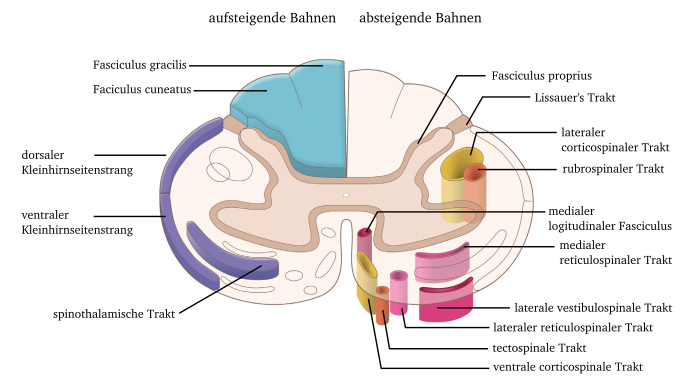
\includegraphics[width = \textwidth] {pictures/somatosensory/aufabsteigendeBahnen_Rueckenmark.png}
    \caption[Auf- und Absteigende Bahnen im Rückenmark]{\textbf{Auf- und Absteigende Bahnen im Rückenmark}\\ Zur besseren Veranschaulichung der Bahnen sind die Bahnen in der Abbildung nach absteigenden Bahnen auf der linken Seite und absteigenden Bahnen auf der rechten Seite aufgeteilt. Beide Gruppen kommen jeweils gespiegelt auch auf der anderen Seite vor.}
    \label{fig:bahnen_rueckenmark}
\end{figure}

\subsubsection{Medulla}

Die Axone des \textit{Fasciculus~gracilis} terminieren im \textit{Nucleus~gracilis} in der Medulla. Auf gleicher Ebene der Medulla enden auch die Axone des \textit{Fasciculus~cuneatus} im \textit{Nucleus~cuneatus}. \textcolor{red}{Hier kann gut ein Bild der medulla eingefügt werden auf dem man die beiden Nuclei sieht und auf welcher ebene sie mit anderen markanten Strukturen der Medulla liegen. vllt gibt es ja auch noch ein bild auf dem gleichzeitig der mediale leminiscus zu sehen ist. Ich sollte auf jedenfall dann beschreiben wie wo sie zu finden sind welche strukturen auch noch dort liegen und anhand was man überhaupt weis dass das die medulla ist -- ventrikel!!!!!}


Beide Nuclei sind zylindrisch geformt und in rostrocaudaler Richtung ausgedehnt. Die afferenten Neuronen aus einer Hautregion enden in der rostrocaudalen Ausdehnung auf einer Linie und verschiedene Hautregionen werden lateral-medial repräsentiert. Die somatosensorische Repräsentation auf dieser Ebene gleicht einem auf dem Rücken liegenden kopflosen Homunculus. Dabei liegen die distalen Körperregionen lateral und die proximalen Hautregionen medial in den Nuclei. Die taktilen und propriozeptiven Informationen des Kopfes werden in angrenzenden \textit{Nucleus principalis nervi trigemini} repräsentiert \cite[Kap.~22]{kandel2013principles}. 

\begin{itemize}

    \item The gracile and cuneate nuclei are shaped like sau-
sages with a rostrocaudal orientation. Primary afferent
fibers terminate on neurons throughout the rostrocau-
dal extent of each nucleus so that a rod-like collection of
cells extending the length of the nucleus represents one
small skin region, and the neurons in any cross section
represent the entire body. The somatic representation
in that neural map is of a headless homunculus lying
on his back with his sacrum toward the midline and his
hands and feet extended dorsally. Tactile and proprio-
ceptive information from the head, face, and mouth is
represented in the adjacent principal trigeminal nucleus.

    \item Axons of neurons in the dorsal column nuclei form the medial lemniscus, which crosses the midline in the medulla and is joined medially by the homologous projection from the trigeminal nuclei. \cite{kandel2013principles} p.492
    \item Cutaneous information from the dorsal column
    and trigeminal nuclei enters the lateral and medial
    ventral posterior nuclei of the thalamus, which form
    a single functional entity. Proprioceptive information
    enters the superior ventral posterior nucleus, which
    lies just above the other two \cite{kandel2013principles} p.493-494
\end{itemize}

\begin{figure}
    \centering
    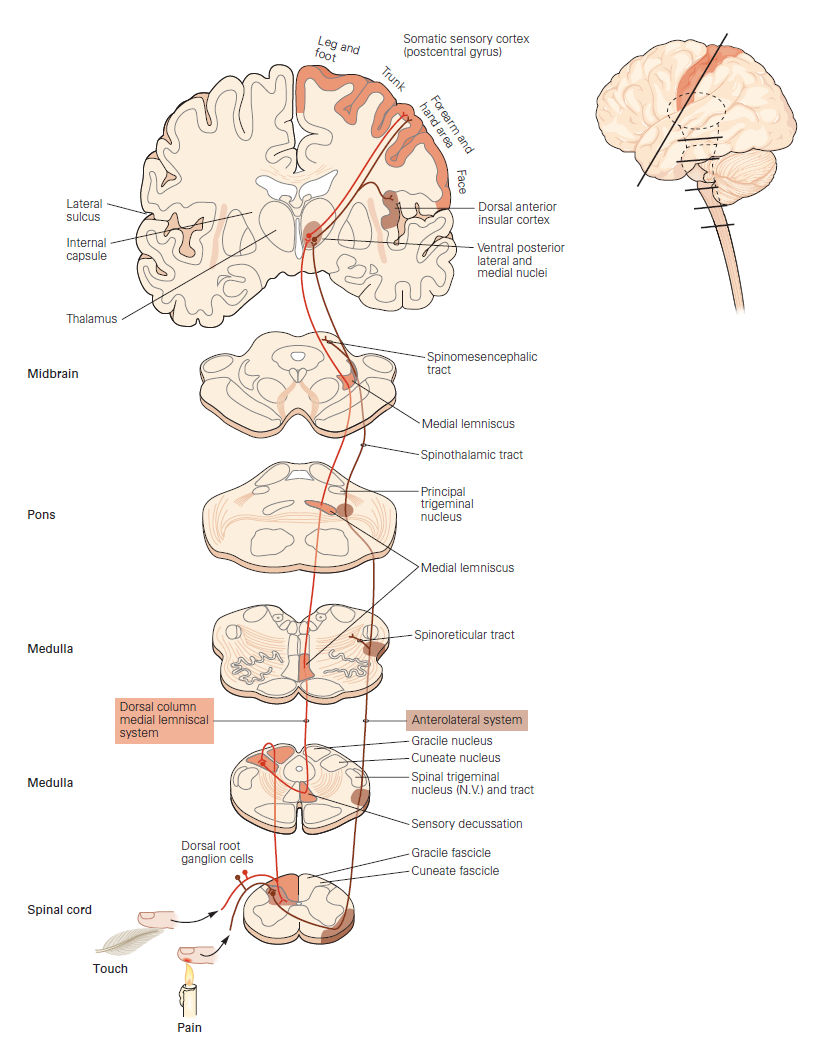
\includegraphics{pictures/somatosensory/pathway_somatosensory2.png}
    \caption[Aufsteigende Bahnen der Somatosensorik]{\textbf{Aufsteigende Bahnen der Somatosensorik}\\
    Die aufsteigenden Bahnen der Somatosensorik sind getrennt in das lemniskale (rot) und das anterolaterale (braun) System. Beginnend im Rückenmark bis zu zum primären somatosensorischen Cortex posterior vom \textit{Sulcus centralis}.\textcolor{red}{genauere beschreibung der einzelnen Sationen???}\\
    \cite[Kap.~22]{kandel2013principles}}
    \label{fig:somato_pathway}
\end{figure}
    
\subsubsection{Schmerz und Temperatursinn (anterolaterales System)}
Der Schmerz- und Temperatursinn hat vor allem eine schützende Funktion auf unseren Körper. Er warnt uns vor Verletzungen oder zu großer Hitze, worauf wir dann reflexartig reagieren und zurückweichen oder die Verletzung behandeln. Der Schmerz \textcolor{red}{entspringt} von den somatosensorischen Strukturen in der Haut und wird von dort zu den höheren Gehirnarealen weitergeleitet. 
Die meisten der Nozizeptoren sind einfache Nervenendigungen primärer sensorischer Faser und können generell in drei Gruppen eingeteilt werden, die thermischen, mechanischen und polymodalen Nozizeptoren \textcolor{red}{Kapitel} \citep{kandel2013principles}. Auch die Zellkörper der Nozizeptoren des Körpers liegen im dorsalen Wurzelganglion und terminieren im Hinterhorn des jeweiligen Segments.  Ihre Synapsen konzentrieren sich in den Schichten I, IV, V, VII, und X des Hinterhorns \cite[Kap.~25]{paxinos2014rat}.
Diese synaptische Verbindung verbindet die Nozizeptoren mit den spinothalamischen Neuronen. Wie der Name dieser Neuronen schon sagt ziehen die Neuronen vom Rückenmark bis in den Thalamus. Die Zellkörper der Neurone liegen in der grauen Substanz des Rückenmarks, während die Axone in der weißen Substanz des Rückenmarks parallel zum Verlauf der Wirbelsäule in Bahnen auf- und absteigen. Die Axone der spinothalamischen Zellen kreuzen auf der Ebene der ersten Synapse die Mittellinie und steigen in der contralateralen weißen Substanz zum lateralen Bereich des Thalamus auf \cite[Kap.~25]{paxinos2014rat}. Bei Ratten bildet die größte Gruppe der spinothalamischen Neurone, die welche auf der Höhe der Halswirbelsäulen der grauen Substanz entspringen.

    
    
\begin{itemize}
    \item protective function, alerting us to injuries that require evasion or treatment. \cite{kandel2013principles}
    \item Pain arising from
    somatic structures is transmitted to higher brain cen-
    ters through the spinothalamic tract pathways in the
    ventral and lateral funiculi of the spinal cord. \cite{paxinos2014rat}
    \item most of these nociceptors
    are simply the free nerve endings of primary sensory
    neurons. There are three main classes of nociceptors—
    thermal, mechanical, and polymodal \cite{kandel2013principles} p.531
    \item whose cell bodies are located in dorsal root
    ganglia or the trigeminal ganglia. The central branches
    of these neurons terminate in the spinal cord in a highly
    orderly manner. Most terminate in the dorsal horn. \cite{kandel2013principles}
    \item The spinothalamic tract origi-
    nates primarily from dorsal horn cells concentrated in
    laminae I, IV, V, VII, and X, i.e., in the marginal zone \cite{paxinos2014rat}
    \item The spi-
    nothalamic cells send their axons across the midline, and
    ascend as the spinothalamic tract in the contralateral white matter to the lateral thalamus. The largest group of spinothalamic neurons in rats is in the upper cervical spinal cord. This cell group projects bilaterally to the thalamus. \cite{paxinos2014rat}
    \item The axons of spinothalamic cells ascending to the lateral thalamus are somatotopically organized. \cite{paxinos2014rat} p.710
    \item Lamina I cells ascend in the lateral funciculus, whereas those from deeper laminae IV, V, and X ascend in the ventral white matter. Spinothalamic tract cells that project to the medial and intralaminar thalamus do so through the
    ventral funiculus
    \item The targets of the axons of spinothalamic cells in the lateral thalamus include the ventral posterolateral (VPL) nucleus and the posterior thalamic nuclear group (Po). Other spinothalamic tract cells target the medial thalamus, including the central lateral nucleus and the nucleus submedius \cite{paxinos2014rat}
    \item The thalamus contains several relay nuclei that participate in the central processing of nociceptive information. Two of the most important regions of the thalamus are the lateral and medial nuclear groups. \cite{kandel2013principles} p.544
    \item zwei andere Wege aus dem peripheren Schmerz und Temperatur Sinn: Spinomesencephalischer Tract und der Spinoreticuläre Tract
    \item It is well known that the spinoreticu-
    lar pathway contributes to descending analgesia and
    autonomic regulation. The spinomesencephalic tract is also involved in noci-ception. However, it is not clear that this tract contributes
    to the sensory-discriminative aspects of pain. Instead, it
    is better suited to contribute to the motivational-affective
    aspects of pain, as well as to trigger activity in descend-
    ing control systems. \cite{paxinos2014rat}
    \item Responses to noxious stimuli have been recorded
    in the primary somatosensory cortex (SmI) of rats
    \cite{paxinos2014rat}
    \item The receptive fields of nociceptive corti-
    cal neurons are larger than those of mechanoreceptive
    neurons, and there are often inhibitory receptive fields.
    Nociceptive neurons are generally located in layers V and VI, whereas mechanoreceptive neurons are mainly
    in layers II–V. \cite{paxinos2014rat}
    \item The cingulate gyrus and insular cortex con-
    tain neurons that are activated strongly and selectively
    by nociceptive somatosensory stimuli (Box 24–1). The
    cingulate gyrus forms part of the limbic system and is
    thought to be involved in processing emotional states
    associated with pain. The insular cortex receives direct
    projections from the thalamus, specifically the medial nuclei and the ventroposterior medial nucleus. Neurons
    in the insular cortex process information about the
    internal state of the body and contribute to the autonomic component of pain responses. \cite{kandel2013principles} p.545
\end{itemize}

\begin{figure}
        \centering
        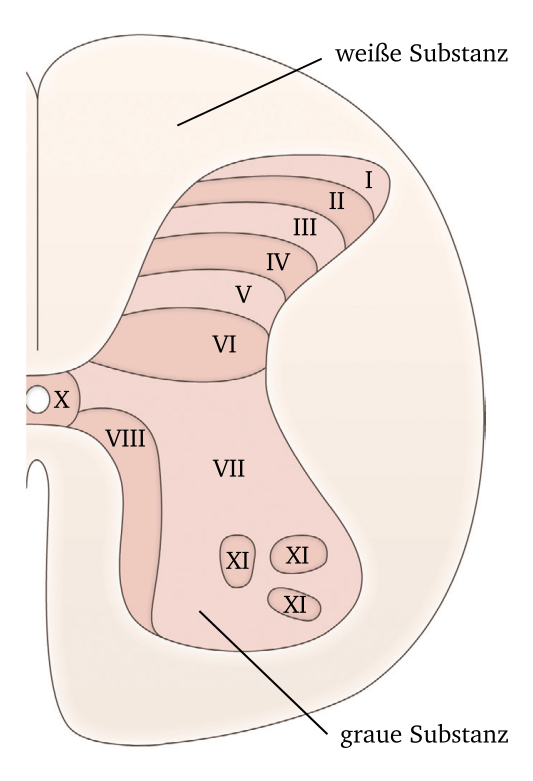
\includegraphics{pictures/somatosensory/graymatter2.png}
        \caption{Caption}
        \label{fig:graymatter}
    \end{figure}


\subsection{Somatosensorik des Kopfes}
\begin{itemize}
    \item Tast, Schmerz und Temperatur am Kopf (trigeminales System)
    \item Primary
afferents for touch on the face and mouth (including the
mystacial vibrissae) travel in the trigeminal nerve (the 5th cranial nerve) to enter the brainstem at the level of
the pons, where they branch and terminate in the prin-
cipal trigeminal nucleus and several subdivisions of the
spinal trigeminal nuclear complex \cite{paxinos2014rat}
\item The axon branches terminating in the principal trigemi-
nal nucleus for touch are analogous to the dorsal column
pathway that terminates in the gracile and cuneate nuclei
for the body \cite{paxinos2014rat}
\item
\end{itemize}
\subsection{(Viscerosensorik)}

\newpage
\section{Spezielle sensorische Bahnen}
% verweis auf dieses Kapitel mit \ref{sec:spezsens}
\label{sec:spezsens}
Die speziellen sensorischen Bahnen umfassen unter anderem die Hörbahn, die Sehbahn und die Riechbahn, womit sich in diesem Kapitel vor allem beschäftigen wird. Diese drei speziellen sensorischen Bahnen spielen sowohl bei der Ratte als auch beim Schaf die zentrale Rolle. Es gibt weiter spezialisierte Sinne wie zum Beispiel den elektrischen Sinn bei Fischen, die beiden chemischen Sinne für Geruch und Geschmack und der Magnetsinn bei Zugvögeln \cite{smith2008biology}. Diese werden nicht in dieser Zusammenfassung behandelt, spielen aber bei anderen Tierarten eine tragende Rolle und sollten aus diesem Grund hier kurz erwähnt werden.

\subsection{Hörbahn}

Die Funktion unserer Ohren ist die Energie eines akustischen Signals von der Außenwelt einzufangen und von einem mechanischen Signal in ein elektrisches Signal umzuwandeln. Diese Umwandlung findet an den inneren Haarsinneszellen in der Cochlea statt. Dort wird durch die Auslenkung der Haarbündel an den inneren Haarsinneszellen (eng.: inner hair cell IHC) die Zelle depolarisiert oder hyperpolarisiert je nach Auslenkungsrichtung. 
\textcolor{red}{Verbindung von IHC to spiral ganglion cell}
\\
\\
Die Spiralganglien verdanken ihren Namen der spiralförmigen Struktur der Cochlea der sie folgen. Sie formen einen Teil des Hirnnerves VIII, der auch Nervus vestibulocochlearis genannt wird. The afferent pathways from the human cochlea
        reflect the functional distinction between inner and
        outer hair cells. At least 90\% of the spiral ganglion
        cells terminate on inner hair cells (Figure 30–17). Each
        axon contacts only a single inner hair cell, but each cell
        directs its output to several nerve fibers, on average
        nearly 10.

\begin{itemize}
    \item Funktion of the ear
    \begin{itemize}
        \item each of our ears must capture this energy, transmit it ot the receptor organ and trancduce it into electrical signals suitable for neural analysis. \cite{kandel2013principles}
        \item von einem mechanischen stimulus zu einem chemischen und dann zu einem elektrischen signal
        \item von den inneren Haarzellen zu den Spiralganglia die deswegen so heißen weil sie der spiralstruckture der cochlea folgen \cite{kandel2013principles}
        \item affrent und efferenter weg in und aus der cochlear wie viel prozent 
        \item The central processes of these bipolar neu-
        rons form the cochlear division of the vestibulococh-
        lear nerve (cranial nerve VIII). Because this ganglion
        follows a spiral course within the bony core of the
        cochlea, it is also called the spiral ganglion. Approxi-
        mately 30,000 ganglion cells innervate the hair cells of
        each inner ear.
        The afferent pathways from the human cochlea
        reflect the functional distinction between inner and
        outer hair cells. At least 90\% of the spiral ganglion
        cells terminate on inner hair cells (Figure 30–17). Each
        axon contacts only a single inner hair cell, but each cell
        directs its output to several nerve fibers, on average
        nearly 10.
        \item The patterns of efferent and afferent connections
        of cochlear hair cells are complementary. Mature inner
        hair cells do not receive efferent input; just beneath
        these cells, however, are extensive axo-axonic synaptic
        contacts between efferent axon terminals and the end-
        ings of afferent nerve fibers. In contrast, efferent nerves
        have extensive connections with outer hair cells on their
        basolateral surfaces. Each outer hair cell receives input
        from several large efferent terminals, which fill the space
        between the cell’s base and the associated Deiters’s cell.
        \item Cochlear Nerve Fibers Encode Stimulus Frequency
        and Intensity
        \end{itemize}
        
    \item Nucleus cochleraris: lateral an der Medulla, ipsilaterale Repräsentation
    \begin{itemize}
        \item terminierung der inneren haarzellen in cochlear nucleus 
        \item tonotopie 
        \item ipsilaterale monoaurale verschaltung
        \item function des cochlaear nucleus
        \item weiter verschaltung: großteil in die obere olive, ein kleiner teil direkt in den lateralen leminiscus und dessen nuclei 
    \end{itemize}
    \item obere Olive
    \begin{itemize}
        \item gesamte nuclei der oberen olive für auditorische verarbeitung (welches sind die anderen kerne??)
        \item function: binaurale verschaltung integration von beiden ohren führt zu richtungs hören
        \item laterale obere olive und mntb für Interaurale intensitäts diffrenz
        \item mediale obere olive für interaurale zeit diffrenz ( tielfe töne) warum bei ratten nochmal kleiner???
        \item wo gehen die zellen dann genau hin
    \end{itemize}
    \item lateraler Lemniscus
    \begin{itemize}
        \item nerven aus der oberen olive ziehen durch den nervenstrang der lateraler leminiscus heißt in den inferior colliculus aber manche sind nochmal zwischen geschaltet in den kernen des lateralen leminiscus ( gibts da ihrgend eine regel oder aufteilung welche verschaltet sind und welche nicht??)
        \item was ist dann der grund für die verschaltung und welche funktion hat der laterale leminiscus ????
    \end{itemize}
    \item Colliculus Inferior
    \begin{itemize}
        \item 
    \end{itemize}
    \item Medial geniculate nucleus
\end{itemize}

\subsection{Sehbahn}
\begin{itemize}
    \item eye
    \begin{itemize}
        \item kurzer überblick über die entwicklung des auges in der embryonal entwicklung retina aus dem diencephalon
        \item auf grund der evolutionären Entwicklunf ein "inverted" auge wesswegen die retina und die photorezeptoren nach innen weg vom licht gerichtet sind
        \item formung der retina: \cite{smith2008biology} p.287
        \item retinale zellen Stäbchen und zäpfchen und dann bipolar zellen und Ganglienzellen 
        \item vllt was zu den rezeptifen feldern
    \end{itemize}
    \item visual pathway
    \begin{itemize}
        \item 3 verschiedene wege ( vorlesung von oswald IN)
        \item wie heißen die von führen sie hin und wir konzentrieren uns auf einen zentralen und warum
    \end{itemize}
    \item optic nerve von der Retina zum Chiasma opticum
    \item Optic chiasm    \index{Optic chiasm}
    \begin{itemize}
        \item Semidecussation  \index{Decussation!Semi-}
        \item ganglienzellen von der nasalen/medialen seite des auges kreuzen am optic chiasm auf die andere seite des gehirns wärend die laterale seite des auges auf der selben seite weiter projezieren
        ßitem keine verschaltung im optischen chiasma sondern nur eine kreuzung der ganglien zellen
        \item danach optic tract
    \end{itemize}
    \item Optic tract \index{Optic tract}
    \item LGN: nicht gestreift, hinterer Teil das Thalamus \index{Thalamus}, auf Höhe des superior colliculus \index{SC!Superior culliculus}
    \begin{itemize}
        \item lateral am Diencephalon \index{Diencephalon} vorbei
        \item posteriorer part des thalamus
        \item aufbau des LGN unterschied zwischen primaten (6 Schichten) und Ratten bzw. Schafen
        \item kurz was zur funktion der verschaltung auf der ebene ( vllt etwas zu den rezeptive fields aber dann auch schon auf der ebene der retina erwähnen)
        \item von LGN über die optic radiation (welche nicht in den schnitten sichtbar ist) ruaf in den neocortex und in V1 
    \end{itemize}
    \item Magnifikationsfaktor = Dichte der Zellen und wie sie verschaltet sind
    \\
\end{itemize}
\subsection{(Riechbahn)}
\begin{itemize}
    \item vom olfactorischen bulb über den olfactorischen trakt zu einerm der ältesten teile des neocortex zum Pyriformen lappen
    \item weitere neuronen führen dann zum thalamus un die weitern stränge dann in den orbitofrontal lobe \cite{smith2008biology} 
    \item eventuell Dopaminerge Bilder
\end{itemize}

\newpage
\section{Motorische Kerngebiete und Bahnen}
\subsection{Motorische Kerngebiete}
\subsection{Motorische Bahnen zum Hirnstamm}
\subsection{Motorische Bahnen zum Rückenmark}
\begin{itemize}
    \item laterales System: corticospinaler Trakt
    \item laterales System: rubrospinaler Trakt
    \item mediales System: reticulospinaler Trakt (medial,lateral)
    \item mediales System: vestibulospinaler Trakt
\end{itemize}
\subsection{Kleinhirn}
\begin{itemize}
    \item Vestibulocerebellum, Spinocerebellum, Corticocerebellum 
    \item Schichtung
    \item funktionelle Einheiten
    \item Schaltkreise
\end{itemize}
\subsection{(Motorik der Kopfmuskulatur)}
\subsection{(Motorik der Augen)}

\newpage
\section{Integrative Systeme}
\subsection{Limbisches System und Hippocampus}
\subsection{Basalganglien}

\newpage
\section{generelle Transmittersysteme (monoaminerge Systeme)}
\section{Quantitative Analyse generelle Transmittersysteme (am Beispiel der catecholaminergen Systeme)}
\subsection{Immunohistochemischer Nachweis catecholaminerger Neurone}
Der immunhistochemische Nachweis catecholaminerger Neurone lässt sich in sechs Einzelschritte unterteilen, diese sind in Material und Methoden auf S.xy zu finden.\newline
1. Quenching\newline
Um eine nicht-spezifische Hintergrundsfärbung durch endogene Peroxidasen zu vermeiden, wird im ersten Schritt durch die Zugabe von Wasserstoffperoxidase eine Reaktion unterbunden. \newline
2. Blocken\newline
Vor der Zugabe des ersten Antikörpers müssen zwei Schritte erfolgen: Zum einen sollen die Antikörper ausschließlich an die spezifischen Bindestellen binden, zum anderen muss den Antikörpern der Zugang zu intrazellulären Antigenen ermöglicht werden.
Um nicht-spezifische Protein-Protein-Interaktion zwischen Antikörpern und Proteinen im zu untersuchenden Gewebe zu unterbinden, werden blockende Poteine hinzuegegeben, die kompetetitv and die unspzifische Bindestelle binden. Hierbei binden Fc-Rezeptoren, welche auf Makrophagen und vielen anderen immunologischen Zellen des Gewebe zu finden sind and das Fc-Ende des Antikörpers und führen somit zur unspezifischen Bindung. 
Um die Antigene des zu untersuchenden Gewebes zugänglich zu machen, muss die Zellmembran vorerst mit Detergenzien bahendelt werden, die die Doppellipidschicht durch Verseifung auflockern - die Permabilisierung.\newline
3. Primärer Antikörper\newline
Der primäre Antikörper besitzt eine Fc-Region, die artspezifisch an unsere Host Bindestelle binder und eine Fab-Region, die an das Epitop des Antigens (Tyrosin-Hydroxylase) bindet.\newline
4. Sekundärer Antikörper\newline
Nun bindet die Fc-Region des ersten Antikörpers and die Fab-Region des zweiten Antikörpers. Der zweite Antikörper ist biotyniliert. \newline
5. Der ABC-Complex\newline
Nachdem das Avidin die biotylinielierte Meerrettich-Peroxidase gebunden hat, kann es nun auch an das biotynilierte Ende des sekundären Antikörpers binden. Dieser Schritt dient der Amplifizerung des Signals.\newline
6. DAB Reaktion\newline
Wasserstoffperoxid bindet and die Meerrettich-Peroxidase und oxidiert das DAB, welches reduziert und nun als bräunliches Edukt vorliegt und somit indirekt die erfolgreiche Bindung and das Antigen sichtbar macht.\newline

\subsection{Lage und Größe der Kerngebiete und Projectionsareale}
\subsection{Dopaminerges und Noradrenegres System}
\begin{itemize}
    \item Incertohypothalamic/nigrostriatal System (Dopamin)
    \item Tuberohypophysial System (Dopamin)
    \item Locus coeruleus (Noradrenalin)
\end{itemize}
\subsection{Größenvergleich der Neurone in \textit{substantia nigra} und \textit{locus coeruleus}}



%%%%%%%%%%%%%%%%%%%%%%%%%%%%%%%%%%%%%%%%%%%%%%%%%%%%%%%%%%5%%
% Bibliography

\newpage
\bibliographystyle{apalike}
\bibliography{references}

%%%%%%%%%%%%%%%%%%%%%%%%%%%%%%%%%%%%%%%%%%%%%%%%%%%%%%%%%%%%%
% Index
\printindex

2n - II optic nerve
3V - 3. Ventrikel\\
3n - III oculomotor nerve\\
4V - 4. Ventrikel\\
5n - V Trigeminus\\
6n - VI nervus abducens\\
\\
Aq - Aquaeductus cerebri\\
Amy - Amygdala\\
ACx - Archicortex\\
\\
CCx - cingulärer Cortex\\
Cu - Nucleus caudatus\\
CPu - Caudoputamen (Striatum)\\
cc - corpus callosum / Balken\\
ChP - choroid plexus\\
Cx - cerebraler Cortex\\
cp - cerebellar peduncle\\
CS - cortical Spine / cortikales Rückenmark\\
Cb - Cerebellum\\
\\
Epi - Epiphyse\\
EO - epithelium olfactorium\\
\\
f - Fornix\\
fi - Fimbria\\
\\
Hi - Hippocampus\\
Hyp - Hypophyse\\
\\
IC - Inferior colliculus\\
ICj - Islands of Calleja\\
\\
LGN - lat. genuculate nuc.\\
lot - lat. olfactory tract\\
LV - lateraler Ventrikel
\\
Med - Medulla\\
MB - mammillary body\\
\\
NCx - Neocortex\\
\\
OB - olfactory bulb / Riechkolben\\
ox - chiasma opticum\\
ot - olfactory tract / olfaktorischer Trakt\\
\\
Pon - Pons\\
PM - Pia mater\\
\\
RF - rhinal fissure\\
\\
SC - Superior colliculus / Colliculus inferior\\
\\
Th - Thalamus\\
Teg - Tegmentum\\
tz - trapezoid body / Trapezkörper\\
TC - Truncus cerebri / Hirnstamm\\
Tu - olfactory tubercle\\
\\
Ve - Velum\\
\\



\end{document}


